% !TeX root = ../main.tex
\chapter{Unidad 6: El mecanismo de la percepción auditiva}

%------------------------------------------------
% OBJETIVO PEDAGÓGICO
%------------------------------------------------

\section*{Objetivo pedagógico}
\noindent\textbf{Objetivo.} Comprender cómo la energía acústica se transforma en señales electroquímicas que el cerebro interpreta como sonido, integrando principios físicos y neurofisiológicos para fundamentar diagnósticos y tratamientos en fonoaudiología, como audiometrías, otoemisiones acústicas (OEA), potenciales evocados auditivos (PEA), implantes cocleares y audífonos osteointegrados (BAHA). Incluye ejemplos clínicos, actividades prácticas, recursos multimedia y ejercicios de autoevaluación.

\noindent\textbf{Pregunta inicial.} ¿Cómo convierte el oído un sonido en una señal que el cerebro puede decodificar? ¿Por qué algunos pacientes perciben mejor las vibraciones a través de los huesos que por el aire? ¡Esta unidad te ayudará a develar los secretos de la audición!

%------------------------------------------------
% PANORAMA GENERAL
%------------------------------------------------

\section{Panorama general}
El sistema auditivo se organiza en cuatro grandes etapas:
\begin{enumerate}
    \item \textbf{Oído externo} – Captación y orientación del sonido.
    \item \textbf{Oído medio} – Adaptación de impedancias y protección.
    \item \textbf{Oído interno} – Análisis frecuencial y transducción mecano-eléctrica.
    \item \textbf{Vía auditiva central} – Procesamiento binaural y percepción cortical.
\end{enumerate}
Cada etapa introduce ganancias y pérdidas que permiten identificar patrones de hipoacusia conductiva, sensorioneural o retrococlear.

\begin{figure}[h]
    \centering
    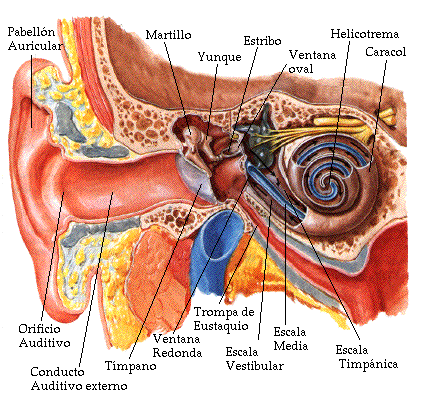
\includegraphics[width=0.8\textwidth]{figures/oido.png}
    \caption{Esquema del sistema auditivo, mostrando el oído externo, medio, interno y la vía auditiva central.}
    \label{fig:sistema_auditivo}
\end{figure}

% Nota: Reemplaza 'esquema_sistema_auditivo.jpg' con el nombre de tu archivo de imagen.

%------------------------------------------------
% OÍDO EXTERNO
%------------------------------------------------

\section{Oído externo: amplificación pasiva y orientación}
\subsection{Pabellón auricular}
El pabellón actúa como una antena direccional que filtra y amplifica frecuencias clave del habla (2–4 kHz). Su geometría genera \textit{notches} espectrales dependientes de la altura de la fuente, brindando pistas para la localización vertical del sonido.

\begin{quote}
    \textbf{Ejemplo clínico.} En casos de \emph{otia microtia} o malformaciones del pabellón, la pérdida de ganancia en altas frecuencias (2–4 kHz) afecta la discriminación de consonantes fricativas, como /s/ y /f/, esenciales para la inteligibilidad del habla.
\end{quote}

% Sugerencia: Incluir una figura del pabellón auricular mostrando los notches espectrales (e.g., \includegraphics[width=0.5\textwidth]{figures/pabellon_notches.jpg}).

\subsection{Canal auditivo externo (CAE)}
El CAE, con una longitud promedio de 27 mm, se comporta como un tubo resonador cerrado, con una frecuencia de resonancia alrededor de 3.2 kHz:
\[
f_{\mathrm{res}} = \frac{c}{4\ell} \approx \frac{343}{4 \cdot 0.027} \approx 3.2 \, \text{kHz}.
\]
Este efecto aporta entre 10 y 15 dB de ganancia en ese rango.

\begin{quote}
    \textbf{Actividad práctica.} Usa un generador de tonos a 3000 Hz (puedes emplear una app como Audacity). Observa la diferencia de sonoridad al tapar parcialmente el pabellón o al ocluir el CAE con un algodón. Opcional: graba el tono y analiza su espectro en Audacity.
\end{quote}

%------------------------------------------------
% OÍDO MEDIO
%------------------------------------------------

\section{Oído medio: adaptación de impedancias y protección}
\subsection{Transformador de impedancia acústica}
El oído medio adapta las impedancias para transferir eficientemente la energía sonora del aire al líquido del oído interno. La membrana timpánica (~60 mm$^2$) concentra la energía en la ventana oval (~3 mm$^2$), logrando una relación de 20:1. Esto, junto con la acción de palanca de la cadena osicular (1.2:1), amplifica la presión sonora, con máxima eficiencia a 1 kHz.

% Sugerencia: Incluir un esquema de la cadena osicular (e.g., \includegraphics[width=0.6\textwidth]{figures/cadena_osicular.jpg}).

\subsection{Reflejo estapedial}
Sonidos $>$ 90 dBSPL activan el músculo del estribo (latencia $\approx$ 50 ms), aumentando la impedancia para proteger la cóclea. No es efectivo ante impulsos breves (e.g., disparos). Su evaluación mediante timpanometría es clave para diagnosticar disfunciones, como en otosclerosis o lesiones del nervio facial.

\begin{quote}
    \textbf{Ejemplo clínico.} En otosclerosis, la ausencia o alteración del reflejo estapedial puede indicar fijación del estribo, observable en la timpanometría.
\end{quote}

%------------------------------------------------
% AUDICIÓN POR VÍA ÓSEA
%------------------------------------------------

\section{Audición por vía ósea}
Por encima de 50 dBSPL, las vibraciones craneales excitan el oído interno por tres rutas:
\begin{enumerate}
    \item \textbf{Inercial}: oscilación diferencial de la cadena osicular.
    \item \textbf{Compresiva}: deformación de la cápsula coclear que genera desplazamiento de perilinfa.
    \item \textbf{Osseo-timpánica}: vibración del CAE que induce movimiento timpánico.
\end{enumerate}
Este principio se aplica en audífonos osteointegrados (BAHA) y pruebas audiométricas de conducción ósea.

\begin{quote}
    \textbf{Actividad práctica.} Compara la percepción de un diapasón (vía ósea, colocado en la mastoides) con un tono por vía aérea (auriculares). Describe las diferencias en intensidad y claridad.
\end{quote}

% Sugerencia: Incluir un esquema de las rutas de conducción ósea (e.g., \includegraphics[width=0.5\textwidth]{figures/conduccion_osea.jpg}).

%------------------------------------------------
% OÍDO INTERNO
%------------------------------------------------

\section{Oído interno: análisis frecuencial y transducción}
\subsection{Arquitectura coclear y tonotopía}
La membrana basilar varía de 150 µm (base) a 450 µm (ápex). Su rigidez decreciente crea un \emph{mapa tonotópico}: 20 kHz en la base, 20 Hz en el ápex (curva de Greenwood). Cada tono activa selectivamente un segmento de ~1 mm.

% Sugerencia: Incluir un esquema de la cóclea desenrollada mostrando el mapa tonotópico (e.g., \includegraphics[width=0.7\textwidth]{figures/cochlea_tonotopia.jpg}).

\subsection{Órgano de Corti y electromotilidad de las CCE}
Las células ciliadas externas (CCE), gracias a la proteína \emph{prestina}, se contraen o alargan en microsegundos, amplificando las vibraciones de la membrana basilar hasta 40 dB y mejorando la selectividad de frecuencias.

\subsection{Evento mecano-eléctrico}
Cuando las estereocilias se mueven más de 10 nm, se abren canales (\textit{tip-links}) que permiten la entrada de iones K$^+$ desde la endolinfa (+80 mV), cambiando el voltaje de la célula (de –70 a 55 mV) y liberando glutamato hacia las neuronas aferentes.

% Sugerencia: Incluir una figura del órgano de Corti con las estereocilias y tip-links (e.g., \includegraphics[width=0.5\textwidth]{figures/organo_corti.jpg}).

%------------------------------------------------
% VÍA AUDITIVA CENTRAL Y PROCESAMIENTO BINAURAL
%------------------------------------------------

\section{Procesamiento binaural y vía auditiva central}
\subsection{Códigos binaurales}
\begin{itemize}
    \item \textbf{ITD} (\emph{Interaural Time Difference}): diferencia de tiempo/fase $<$1.5 kHz, procesada en el núcleo olivar superior medial (MSO).
    \item \textbf{ILD} (\emph{Interaural Level Difference}): sombra acústica $>$3 kHz, procesada en el núcleo olivar superior lateral (LSO).
\end{itemize}
Ambas pistas, combinadas con los \textit{notches} del pabellón, permiten localizar sonidos en 3D con una precisión angular de 1° en azimut.

\begin{quote}
    \textbf{Actividad práctica.} Con auriculares, escucha el efecto binaural \href{https://www.youtube.com/watch?v=IUDTlvagjJA&ab_channel=LovelyVirus}{“Virtual Barber Shop”}. Identifica cómo varían ITD e ILD cuando la fuente “rodea” tu cabeza. Opcional: prueba tapando un oído y describe el cambio en la percepción espacial.
\end{quote}

% Sugerencia: Incluir un diagrama de la cabeza mostrando ITD e ILD (e.g., \includegraphics[width=0.5\textwidth]{figures/binaural_cues.jpg}).

%------------------------------------------------
% APLICACIONES CLÍNICAS
%------------------------------------------------

\section{Aplicaciones clínicas principales}
\begin{itemize}
    \item \textbf{Audiometría aérea y ósea}: define el patrón de pérdida (conductiva, mixta o sensorioneural).
    \item \textbf{Otoemisiones acústicas}: TEOAE y DPOAE para cribado neonatal y monitoreo ototóxico.
    \item \textbf{Potenciales evocados auditivos} (PEA): valoración de latencias onda I–V, útil en diagnóstico retrococlear.
    \item \textbf{Impedanciometría}: timpanometría + reflejo estapedial.
    \item \textbf{Implante coclear}: estimulación eléctrica directa respetando la tonotopía, con mapeo de electrodos (20–8000 Hz).
\end{itemize}

\begin{quote}
    \textbf{Caso clínico.} Un neonato no responde al cribado con OEA. La PEA muestra latencias normales. ¿Qué pruebas adicionales recomendarías? ¿Qué tipo de hipoacusia sospecharías?
\end{quote}

% Sugerencia: Incluir un ejemplo de audiograma (e.g., \includegraphics[width=0.6\textwidth]{figures/audiograma.jpg}).

%------------------------------------------------
% EJEMPLOS PRÁCTICOS
%------------------------------------------------

\section{Ejemplos prácticos}
\begin{enumerate}
    \item \textbf{Ganancia del oído medio.} $A_t=60 \, \text{mm}^2$, $A_{vo}=3 \, \text{mm}^2$, palanca $1.2:1$. $G = 20\log_{10}\left(\frac{60}{3} \cdot 1.2\right) \approx 27.6 \, \text{dB}$.
    \item \textbf{Reflejo estapedial vs. impulso breve.} Un disparo de 120 dB, 0.1 ms, no desencadena el reflejo; riesgo de trauma acústico.
    \item \textbf{ITD máximo.} Calcula el retardo interaural máximo para una cabeza de 18 cm de diámetro:
    \[
    \Delta t_{\max} = \frac{d}{c} = \frac{0.18}{343} \approx 525 \, \mu\text{s}.
    \]
\end{enumerate}

%------------------------------------------------
% EJERCICIOS DE AUTOEVALUACIÓN
%------------------------------------------------

\section{Ejercicios de autoevaluación}
\begin{enumerate}
    \item ¿Cómo afecta la pérdida de CCE a la selectividad frecuencial? Relaciona con el ensanchamiento de las \emph{tuning curves}.
    \item Explica la diferencia entre ITD e ILD y en qué rangos de frecuencia predominan.
    \item Describe el principio de funcionamiento de un BAHA.
    \item Interpreta un audiograma con vía aérea 40 dB HL y vía ósea 10 dB HL en 500–2000 Hz.
    \item Un paciente de 60 años presenta pérdida auditiva bilateral en altas frecuencias y ausencia de reflejo estapedial. ¿Qué pruebas recomendarías y qué tipo de hipoacusia sospecharías?
\end{enumerate}

%------------------------------------------------
% RECURSOS Y BIBLIOGRAFÍA
%------------------------------------------------

\section{Recursos multimedia y bibliografía}
\begin{itemize}
    \item Video: \href{https://www.youtube.com/watch?v=jAc8A5NhJKk&ab_channel=NationalInstitutesofHealth%28NIH%29}{``El viaje del sonido al cerebro''}.
    \item Simulación: \emph{Sound Localization Demo} (MIT \slash HRTF).
    \item App: \emph{Audacity}. Visualización espectral.
    \item Simulación interactiva: \emph{Hearing Simulation} (Universidad de Minnesota, disponible en línea).
    \item Libro: Schnupp and Nelken, \emph{Auditory Neuroscience}, cap. 1–6.
    \item Libro: Pickles, \emph{Physiology of Hearing}, 4ª ed.
\end{itemize}

%------------------------------------------------
% GLOSARIO
%------------------------------------------------

\section*{Glosario}
\begin{description}
    \item[\textbf{ITD}] (\emph{Interaural Time Difference}): diferencia temporal entre oídos.
    \item[\textbf{ILD}] (\emph{Interaural Level Difference}): diferencia de nivel entre oídos.
    \item[\textbf{Prestina}] Proteína motora de las CCE responsable de la electromotilidad.
    \item[\textbf{BAHA}] (Bone-Anchored Hearing Aid): prótesis osteointegrada.
    \item[\textbf{Tuning curve}] Curva de sintonía neural.
    \item[\textbf{Tonotopía}] Organización espacial de frecuencias en la cóclea.
    \item[\textbf{Notches espectrales}] Reducciones en el espectro sonoro causadas por la geometría del pabellón.
\end{description}

%------------------------------------------------
% RESUMEN
%------------------------------------------------

\section*{Resumen}
\begin{itemize}
    \item \textbf{Oído externo}: amplifica 2–4 kHz y aporta pistas espaciales.
    \item \textbf{Oído medio}: transformador de impedancias (+27 dB) y protección.
    \item \textbf{Oído interno}: tonotopía y amplificación activa.
    \item \textbf{Vía central}: integra ITD/ILD y genera la percepción consciente.
    \item \textbf{Clínica}: audiometría, OEA, PEA, BAHA, implantes cocleares.
\end{itemize}

\bigskip
\noindent\emph{Conclusión.} La audición emerge de un delicado encadenamiento de procesos físicos, mecánicos, eléctricos y cognitivos. Conocerlos habilita intervenciones clínicas efectivas y fundamenta el diseño de tecnologías auditivas.





%%%%%%%%%%%%%%%%%%%%%%%%%%%%%%%%%%%%%%%%%%%%%%%%%%%%%%%%%%%%%%%%%%%%%%%%%%%%%%%%%%%%%%%%%%%%%%%%%%
